\documentclass[
../../AuD-Zusammenfassung.tex,
]
{subfiles}

\externaldocument[ext:]{../../AuD-Zusammenfassung}
% Set Graphics Path, so pictures load correctly
\graphicspath{{../../}}

\begin{document}
\section{Grundlegende Datenstrukturen}
\subsection{Stacks}
Stacks operieren unter dem "First in - Last out" (FILO) Prinzip. Ähnlich zu einem Kartendeck, wo die unterste (Erste Karte) die ist, die als letztes gezogen wird. \\
Stacks werden normalerweise mit den folgenden Funktionen erstellt:
\begin{itemize}
    \item \texttt{new(n)}: Erstellt einen neuen Stack.
    \item \texttt{isEmpty}: gibt an ob der Stack leer ist.
    \item \texttt{pop}: gibt das oberste Element des Stacks zurück und enfernt es vom Stack.
    \item \texttt{push(k)}: Fügt \texttt{k} auf den Stack hinzu
\end{itemize}
Eine mögliche Implementation auf Grundlage eines Arrays wäre:
\lstinputlisting[language=Java]{Code/Stack.java}

Push und Pop schmeißen Fehlermeldung wenn Stack leer bzw. voll ist. Oft als Stack underflow und Stack overflow benannt. Hier wär es automatisch IndexOutOfBounds.\\ Oft werden Stacks auch mit variabler Größer implementiert. Dies kann über verschiedene Wege passieren, zum Beispiel Kopieren des arrays in einen größeren Array oder implementation über mehrere Arrays (z.B. über Linked List). Häufig wird das erstere so implementiert, dass der Array in einen Array mit doppelter Größe kopiert wird.\\
\vspace{20pt}\\
\begin{minipage}[t]{0.33\textwidth}
    \centering
    \begin{tikzpicture}[
        every node/.style={draw,minimum width=30pt, minimum height=20pt, rectangle, rounded corners, text centered},
        invis/.style={draw=none},
        node distance = 10pt,
    ]
        \node[invis](bottom){};
        \node[invis, above =of bottom](mid){};
        \node[invis, above =of mid](top){};
        \node[at=(bottom)](4){4};
        \node[at=(mid)](6){6};
        \node[at=(top)](8){8};

        \coordinate(hulltopleft) at ($(top.north west) + (-5pt, 5pt)$);
        \coordinate(hulltopright) at ($(top.north east) + (5pt, 5pt)$);
        \coordinate(hullbottomleft) at ($(bottom.south west) + (-5pt, -5pt)$);
        \coordinate(hullbottomright) at ($(bottom.south east) + (5pt, -5pt)$);
        \draw[ultra thick, rounded corners] (hulltopleft) rectangle (hullbottomright);
        \draw[line width=3pt, white] (hulltopleft) to (hulltopright);
    \end{tikzpicture}
    \captionof*{figure}{Example Stack}
\end{minipage}
\begin{minipage}[t]{0.33\textwidth}
    \centering
    \begin{tikzpicture}[
        every node/.style={draw,minimum width=30pt, minimum height=20pt, rectangle, rounded corners, text centered},
        invis/.style={draw=none},
        node distance = 10pt,
    ]
        \node[invis](bottom){};
        \node[invis, above =of bottom](mid){};
        \node[invis, above =of mid](top){};
        \node[at=(bottom)](4){4};
        \node[at=(mid)](6){6};
        \node[above right =of top, magenta](8){8};

        \coordinate(hulltopleft) at ($(top.north west) + (-5pt, 5pt)$);
        \coordinate(hulltopright) at ($(top.north east) + (5pt, 5pt)$);
        \coordinate(hullbottomleft) at ($(bottom.south west) + (-5pt, -5pt)$);
        \coordinate(hullbottomright) at ($(bottom.south east) + (5pt, -5pt)$);
        \draw[ultra thick, rounded corners] (hulltopleft) rectangle (hullbottomright);
        \draw[line width=3pt, white] (hulltopleft) to (hulltopright);
        \draw[very thick, ->, bend left=30] (top.center) to (8.west);
    \end{tikzpicture}
    \captionof*{figure}{Pop}
\end{minipage}
\begin{minipage}[t]{0.33\textwidth}
    \centering
    \begin{tikzpicture}[
        every node/.style={draw,minimum width=30pt, minimum height=20pt, rectangle, rounded corners, text centered},
        invis/.style={draw=none},
        node distance = 10pt,
    ]
        \node[invis](bottom){};
        \node[invis, above =of bottom](mid){};
        \node[invis, above =of mid](top){};
        \node[at=(bottom)](4){4};
        \node[at=(mid)](6){6};
        \node[above left =of top, codegreen](1){1};

        \coordinate(hulltopleft) at ($(top.north west) + (-5pt, 5pt)$);
        \coordinate(hulltopright) at ($(top.north east) + (5pt, 5pt)$);
        \coordinate(hullbottomleft) at ($(bottom.south west) + (-5pt, -5pt)$);
        \coordinate(hullbottomright) at ($(bottom.south east) + (5pt, -5pt)$);
        \draw[ultra thick, rounded corners] (hulltopleft) rectangle (hullbottomright);
        \draw[line width=3pt, white] (hulltopleft) to (hulltopright);
        \draw[very thick, <-, bend right=30] (top.center) to (1.east);
    \end{tikzpicture}
    \captionof*{figure}{Push}
\end{minipage}
\newpage
\subsection{Queues}
Queues funktionieren entgegengesetzt zu Stacks. Sie funktionieren nach dem FIFO-Prinzip (First in - First out). Kann als Warteschleife dargestellt werden. Die Person, die sich als erstes anstellt, kommt auch als erstes dran.
Queues werden normalerweise mit den folgenden Funktionen erstellt:
\begin{itemize}
    \item \texttt{new(n)}: Erstellt einen neuen Queue.
    \item \texttt{isEmpty}: gibt an ob der Queue leer ist.
    \item \texttt{enqueue(k)}: Fügt \texttt{k} auf den Queue hinzu
    \item \texttt{dequeue}: gibt das erste Element des Queues zurück und entfernt es vom Queue.
\end{itemize}
Hier ist die Implementation für Queues wie folgt:

\lstinputlisting[language=Java]{Code/Queue.java}
\begin{minipage}[t]{\textwidth}
    \centering
    \begin{tikzpicture}[
        every node/.style={draw,minimum width=30pt, minimum height=20pt, rectangle, rounded corners, text centered},
        invis/.style={draw=none},
        node distance = 10pt,
    ]
        \node[invis](rear){};
        \node[invis, right =of rear](midl){};
        \node[invis, right =of midl](mid){};
        \node[invis, right =of mid](midr){};
        \node[invis, right =of midr](front){};
        \node[at=(front)](4){4};
        \node[at=(midr)](6){6};
        \node[at=(mid)](8){8};
        \node[at=(midl)](1){1};
        \node[below =of rear, invis](descrear){Rear};
        \node[below =of front, invis](descfront){Front};

        \coordinate(hulltopleft) at ($(rear.north west) + (-5pt, 5pt)$);
        \coordinate(hulltopright) at ($(front.north east) + (5pt, 5pt)$);
        \coordinate(hullbottomleft) at ($(rear.south west) + (-5pt, -5pt)$);
        \coordinate(hullbottomright) at ($(front.south east) + (5pt, -5pt)$);
        \draw[ultra thick, rounded corners] (hulltopleft) rectangle (hullbottomright);
        \draw[line width=3pt, white] (hulltopleft) to (hullbottomleft);
        \draw[line width=3pt, white] (hulltopright) to (hullbottomright);
    \end{tikzpicture}
    \captionof*{figure}{Example non-cyclic Queue}
\end{minipage}\\
\vspace{20pt}
\\
\begin{minipage}[t]{0.5\textwidth}
    \centering
    \begin{tikzpicture}[
        every node/.style={draw,minimum width=30pt, minimum height=20pt, rectangle, rounded corners, text centered},
        invis/.style={draw=none},
        node distance = 10pt,
    ]
        \node[invis](rear){};
        \node[invis, right =of rear](midl){};
        \node[invis, right =of midl](mid){};
        \node[invis, right =of mid](midr){};
        \node[invis, right =of midr](front){};
        \node[right =of front](4){4};
        \node[at=(midr)](6){6};
        \node[at=(mid)](8){8};
        \node[at=(midl)](1){1};
        \node[below =of rear, invis](descrear){Rear};
        \node[below =of front, invis](descfront){Front};

        \coordinate(hulltopleft) at ($(rear.north west) + (-5pt, 5pt)$);
        \coordinate(hulltopright) at ($(front.north east) + (5pt, 5pt)$);
        \coordinate(hullbottomleft) at ($(rear.south west) + (-5pt, -5pt)$);
        \coordinate(hullbottomright) at ($(front.south east) + (5pt, -5pt)$);
        \draw[ultra thick, rounded corners] (hulltopleft) rectangle (hullbottomright);
        \draw[line width=3pt, white] (hulltopleft) to (hullbottomleft);
        \draw[line width=3pt, white] (hulltopright) to (hullbottomright);
        \draw[very thick, ->] (front.center) to (4.west);
    \end{tikzpicture}
    \captionof*{figure}{Dequeue}
\end{minipage}
\begin{minipage}[t]{0.5\textwidth}
    \centering
    \begin{tikzpicture}[
        every node/.style={draw,minimum width=30pt, minimum height=20pt, rectangle, rounded corners, text centered},
        invis/.style={draw=none},
        node distance = 10pt,
    ]
        \node[invis](rear){};
        \node[invis, right =of rear](midl){};
        \node[invis, right =of midl](mid){};
        \node[invis, right =of mid](midr){};
        \node[invis, right =of midr](front){};
        \node[at=(midr)](6){6};
        \node[at=(mid)](8){8};
        \node[at=(midl)](1){1};
        \node[left =of rear](7){7};
        \node[below =of rear, invis](descrear){Rear};
        \node[below =of front, invis](descfront){Front};
        

        \coordinate(hulltopleft) at ($(rear.north west) + (-5pt, 5pt)$);
        \coordinate(hulltopright) at ($(front.north east) + (5pt, 5pt)$);
        \coordinate(hullbottomleft) at ($(rear.south west) + (-5pt, -5pt)$);
        \coordinate(hullbottomright) at ($(front.south east) + (5pt, -5pt)$);
        \draw[ultra thick, rounded corners] (hulltopleft) rectangle (hullbottomright);
        \draw[line width=3pt, white] (hulltopleft) to (hullbottomleft);
        \draw[line width=3pt, white] (hulltopright) to (hullbottomright);
        \draw[very thick, <-] (rear.center) to (7.east);
    \end{tikzpicture}
    \captionof*{figure}{Enqueue}
\end{minipage}\\
\vspace*{50pt}
\\
\begin{minipage}[t]{\textwidth}
    \centering
    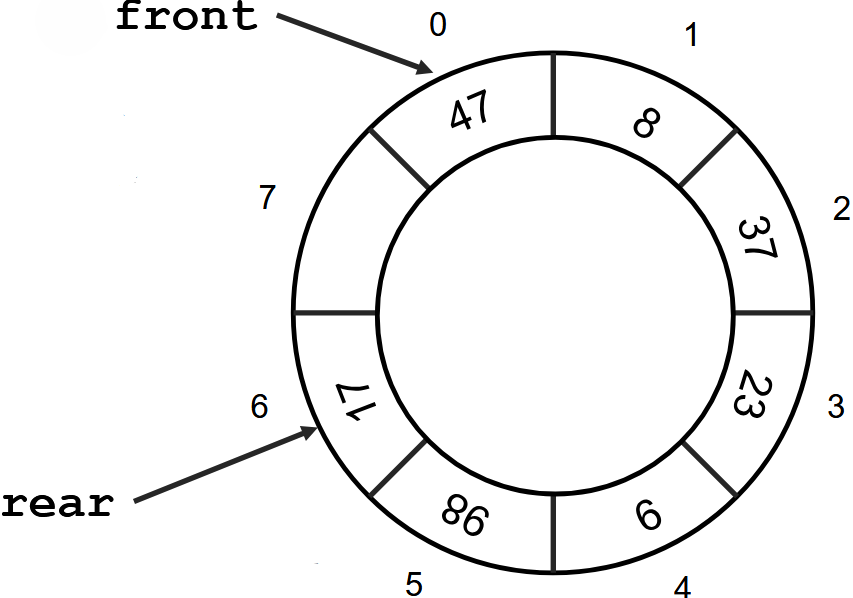
\includegraphics[scale=0.5]{Pics/CyclicQueue.png}
    \captionof*{figure}{Cyclic Queue}
\end{minipage}
\newpage
\subsection{Linked List}
Eine einfache Linked List besteht aus mehreren Elementen, die jeweils immer einen Wert und eine Referenz auf das nächste Element in der Liste haben. Diese Struktur hat den Vorteil, dass sie keine festgelegte Größe hat, das Einfügen in $O(1)$ stattfindet, einfach zu implementieren ist und im Speicher nicht als Block, sondern einzelne Referenzen steht. Eine einfache Linked List kann wie folgt implementiert werden:

\lstinputlisting[language=Java]{Code/LinkedList.java}
Diese Implementation benutzt einen Head und Tail, hat aber nur Referenz für das nächste Element in der Liste. Eine alternative Implementation wäre Tail wegzulassen und den Nodes eine previous-Referenz zu geben. Damit könnte man beim Einfügen das Element vorne an den Head anzuhängen und die neue Node als Head zuzuweisen. \texttt{search} bleibt gleich, bei \texttt{delete} muss lediglich die previous Referenz angepasst werden.
\newpage
\begin{minipage}[t]{\textwidth}
    \centering
    \begin{tikzpicture}[
        every node/.style={draw,minimum width=30pt, minimum height=20pt, rectangle, rounded corners, text centered},
        invis/.style={draw=none},
        every path/.style={draw, very thick},
    ]
    \node[](4){4};
    \node[right =of 4](6){6};
    \node[right =of 6](3){3};
    \node[right =of 3](5){5};
    \node[right =of 5](1){1};
    \node[invis, below =5pt of 4](deschead){Head};
    \node[invis, below =5pt of 1](desctail){Tail};

    \draw[->] (4) to (6);
    \draw[->] (6) to (3);
    \draw[->] (3) to (5);
    \draw[->] (5) to (1);
    

    \end{tikzpicture}
    \captionof*{figure}{Linked List}
\end{minipage}\\
\vspace{20pt}\\
\begin{minipage}[t]{\textwidth}
    \centering
    \begin{tikzpicture}[
        every node/.style={draw,minimum width=30pt, minimum height=20pt, rectangle, rounded corners, text centered},
        invis/.style={draw=none},
        every path/.style={draw, very thick},
    ]
    \node[](4){4};
    \node[right =of 4](6){6};
    \node[right =of 6, magenta](3){3};
    \node[right =of 3](5){5};
    \node[right =of 5](1){1};
    \node[invis, below =5pt of 4](deschead){Head};
    \node[invis, below =5pt of 1](desctail){Tail};

    \draw[->] (4) to (6);
    \draw[->, bend left=45, codegreen] (6.east) to (5.west);
    \draw[->] (3) to (5);
    \draw[->] (5) to (1);
    

    \end{tikzpicture}
    \captionof*{figure}{Delete Outcome}
\end{minipage}
\begin{minipage}[t]{\textwidth}
    \centering
    \begin{tikzpicture}[
        every node/.style={draw,minimum width=30pt, minimum height=20pt, rectangle, rounded corners, text centered},
        invis/.style={draw=none},
        every path/.style={draw, very thick},
    ]
    \node[](4){4};
    \node[right =of 4](6){6};
    \node[right =of 6](5){5};
    \node[right =of 5](1){1};
    \node[invis, below =5pt of 4](deschead){Head};
    \node[invis, below =5pt of 1](desctail){Tail};

    \draw[->] (4) to (6);
    \draw[->] (6) to (5);
    \draw[->] (5) to (1);
    

    \end{tikzpicture}
    \captionof*{figure}{Delete Quasi Outcome}
\end{minipage}
Die 3 Node wird zwar nicht wirklich "gelöscht", allerdings wird die Referenz aus der Liste genommen, wodurch keine Referenz mehr auf diese Node besteht.
\\
\vspace{20pt}
\\
\begin{minipage}[t]{\textwidth}
    \centering
    \begin{tikzpicture}[
        every node/.style={draw,minimum width=30pt, minimum height=20pt, rectangle, rounded corners, text centered},
        invis/.style={draw=none},
        every path/.style={draw, very thick},
    ]
    \node[](4){4};
    \node[right =of 4](6){6};
    \node[right =of 6](5){5};
    \node[right =of 5](1){1};
    \node[right =of 1, codegreen](8){8};
    \node[invis, below =5pt of 4](deschead){Head};
    \node[invis, below =5pt of 8](desctail){Tail};

    \draw[->] (4) to (6);
    \draw[->] (6) to (5);
    \draw[->] (5) to (1);
    \draw[->] (1) to (8);
    

    \end{tikzpicture}
    \captionof*{figure}{Insert of 8}
\end{minipage}
8 wird an tail angehängt und wird dann zum tail
\newpage
\subsection{Binary Search Tree}
Ein Binary Search Tree ist eine Datenstruktur, die aus mehreren Nodes besteht, die jeweils pointer zu drei Nodes besitzt: Left, Right und Parent. \\
Hierbei repräsentiert Left und Right die Nodes, die unter der current Node stehen und Parent die, die über der current Node steht. Dabei ist im Binary Search Tree (Im Gegensatz zum normalen Search Tree) Left immer kleiner als die Node und Right immer größer gleich der Node. \\
Dies erlaubt es Elemente in dem Tree schnell zu finden, da nicht alle Elemente durchlaufen werden müssen, sondern immer nur ein Pfad, bei dem das Element größer/kleiner ist. \\
Ein idealer Binary Search Tree ist so balanziert, dass beide Seiten des Baumes die selbe Anzahl an Knoten besitzen. Dies wäre eine ideale Höhe von $h = \log n$.
Ein schlechter Binary Search Tree allerdings ist unbalanziert, so dass der Worst-Case so aussieht, dass alle Nodes jeweils maximal ein Kind haben. Dies wäre effektiv gleich einer LinkedList.
\lstinputlisting[language=Java, lastline = 30]{Code/BSTree.java}
\begin{minipage}[t]{0.5\textwidth}
    \centering
    \begin{tikzpicture}[
        every node/.style={draw,minimum size=15pt, circle, text centered, thick},
        %every child/.style={edge from parent fork down, -latex},
        node distance = 25pt,
        %forked edge/.style={edge from parent fork down, draw, -latex},
        invis/.style={draw=none},
    ]

    \node[](6){6};
    
    \node[below left =of 6](4){4};
        \node[below left =of 4, xshift=13pt](2){2};

    \node[below right =of 6](8){8};
        \node[below left =of 8, xshift=13pt](7){7};
        \node[below right =of 8, xshift=-13pt](9){9};
        

    \draw[->, thick] (6) to (4);
    \draw[->, thick] (6) to (8);
    \draw[->, thick] (4) to (2);
    \draw[->, thick] (8) to (7);
    \draw[->, thick] (8) to (9);
    \end{tikzpicture}
    \captionof*{figure}{Before insert}
\end{minipage}
\begin{minipage}[t]{0.5\textwidth}
    \centering
    \begin{tikzpicture}[
        every node/.style={draw,minimum size=15pt, circle, text centered, thick},
        %every child/.style={edge from parent fork down, -latex},
        node distance = 25pt,
        %forked edge/.style={edge from parent fork down, draw, -latex},
        invis/.style={draw=none},
    ]

    \node[](6){6};
    
    \node[below left =of 6](4){4};
        \node[below left =of 4, xshift=13pt](2){2};
        \node[below right =of 4, xshift=-13pt, codegreen](5){5};
    \node[below right =of 6](8){8};
        \node[below left =of 8, xshift=13pt](7){7};
        \node[below right =of 8, xshift=-13pt](9){9};
        

    \draw[->, thick] (6.225) to (4.75);
    \draw[->, thick] (6) to (8);
    \draw[->, thick] (4) to (2);
    \draw[->, thick] (8) to (7);
    \draw[->, thick] (8) to (9);

    \draw[->, thick, codegreen] (6.255) to (4.45);
    \draw[->, thick, codegreen] (4) to (5);
    \end{tikzpicture}
    \captionof*{figure}{Insert 5}
\end{minipage}
\newpage
\lstinputlisting[language=Java, firstline = 31, lastline = 61]{Code/BSTree.java}
\begin{minipage}[t]{0.33\textwidth}
    \centering
    \begin{tikzpicture}[
        every node/.style={draw,minimum size=15pt, circle, text centered, thick},
        node distance = 22pt,
        invis/.style={draw=none},
    ]

    \node[](6){6};
    
    \node[below left =of 6](4){4};
        \node[below left =of 4, xshift=13pt](2){2};

    \node[below right =of 6](8){8};
        \node[below left =of 8, xshift=13pt](7){7};
        \node[below right =of 8, xshift=-13pt](9){9};
        

    \draw[->, thick] (6) to (4);
    \draw[->, thick] (6) to (8);
    \draw[->, thick] (4) to (2);
    \draw[->, thick] (8) to (7);
    \draw[->, thick] (8) to (9);
    \end{tikzpicture}
    \captionof*{figure}{Leaf Deletion}
\end{minipage}
\begin{minipage}[t]{0.33\textwidth}
    \centering
    \begin{tikzpicture}[
        every node/.style={draw,minimum size=15pt, circle, text centered, thick},
        node distance = 22pt,
        invis/.style={draw=none},
    ]

    \node[](6){6};
    
    \node[below left =of 6](4){4};
        \node[below left =of 4, xshift=13pt, magenta](2){2};

    \node[below right =of 6](8){8};
        \node[below left =of 8, xshift=13pt](7){7};
        \node[below right =of 8, xshift=-13pt](9){9};
        

    \draw[->, thick] (6) to (4);
    \draw[->, thick] (6) to (8);
    \draw[->, thick, magenta] (4) to (2);
    \draw[->, thick] (8) to (7);
    \draw[->, thick] (8) to (9);
    \end{tikzpicture}
    \captionof*{figure}{Delete 2}
\end{minipage}
\begin{minipage}[t]{0.33\textwidth}
    \centering
    \begin{tikzpicture}[
        every node/.style={draw,minimum size=15pt, circle, text centered, thick},
        node distance = 22pt,
        invis/.style={draw=none},
    ]

    \node[](6){6};
    
    \node[below left =of 6](4){4};

    \node[below right =of 6](8){8};
        \node[below left =of 8, xshift=13pt](7){7};
        \node[below right =of 8, xshift=-13pt](9){9};
        

    \draw[->, thick] (6) to (4);
    \draw[->, thick] (6) to (8);
    \draw[->, thick] (8) to (7);
    \draw[->, thick] (8) to (9);
    \end{tikzpicture}
    \captionof*{figure}{Result}
\end{minipage}

\begin{minipage}[t]{0.33\textwidth}
    \centering
    \begin{tikzpicture}[
        every node/.style={draw,minimum size=15pt, circle, text centered, thick},
        node distance = 22pt,
        invis/.style={draw=none},
    ]

    \node[](6){6};
    
    \node[below left =of 6](4){4};
        \node[below left =of 4, xshift=13pt](2){2};

    \node[below right =of 6](8){8};
        \node[below left =of 8, xshift=13pt](7){7};
        \node[below right =of 8, xshift=-13pt](9){9};
        

    \draw[->, thick] (6) to (4);
    \draw[->, thick] (6) to (8);
    \draw[->, thick] (4) to (2);
    \draw[->, thick] (8) to (7);
    \draw[->, thick] (8) to (9);
    \end{tikzpicture}
    \captionof*{figure}{Half-Leaf Deletion}
\end{minipage}
\begin{minipage}[t]{0.33\textwidth}
    \centering
    \begin{tikzpicture}[
        every node/.style={draw,minimum size=15pt, circle, text centered, thick},
        node distance = 22pt,
        invis/.style={draw=none},
    ]

    \node[](6){6};
    
    \node[below left =of 6, magenta](4){4};
        \node[below left =of 4, xshift=13pt](2){2};

    \node[below right =of 6](8){8};
        \node[below left =of 8, xshift=13pt](7){7};
        \node[below right =of 8, xshift=-13pt](9){9};
        

    \draw[->, thick, magenta] (6) to (4);
    \draw[->, thick] (6) to (8);
    \draw[->, thick] (4) to (2);
    \draw[->, thick] (8) to (7);
    \draw[->, thick] (8) to (9);
    \draw[->, thick, bend right=45, codegreen] (6) to (2);
    \end{tikzpicture}
    \captionof*{figure}{Delete 4}
\end{minipage}
\begin{minipage}[t]{0.33\textwidth}
    \centering
    \begin{tikzpicture}[
        every node/.style={draw,minimum size=15pt, circle, text centered, thick},
        node distance = 22pt,
        invis/.style={draw=none},
    ]

    \node[](6){6};
    
    \node[below left =of 6](2){2};
    
    \node[below right =of 6](8){8};
        \node[below left =of 8, xshift=13pt](7){7};
        \node[below right =of 8, xshift=-13pt](9){9};
        

    \draw[->, thick] (6) to (2);
    \draw[->, thick] (6) to (8);
    \draw[->, thick] (8) to (7);
    \draw[->, thick] (8) to (9);
    \end{tikzpicture}
    \captionof*{figure}{Result}
\end{minipage}

\begin{minipage}[t]{0.33\textwidth}
    \centering
    \begin{tikzpicture}[
        every node/.style={draw,minimum size=15pt, circle, text centered, thick},
        node distance = 22pt,
        invis/.style={draw=none},
    ]

    \node[](6){6};
    
    \node[below left =of 6](4){4};
        \node[below left =of 4, xshift=13pt](2){2};

    \node[below right =of 6](8){8};
        \node[below left =of 8, xshift=13pt](7){7};
        \node[below right =of 8, xshift=-13pt](9){9};
        

    \draw[->, thick] (6) to (4);
    \draw[->, thick] (6) to (8);
    \draw[->, thick] (4) to (2);
    \draw[->, thick] (8) to (7);
    \draw[->, thick] (8) to (9);
    \end{tikzpicture}
    \captionof*{figure}{Complete Node Deletion}
\end{minipage}
\begin{minipage}[t]{0.33\textwidth}
    \centering
    \begin{tikzpicture}[
        every node/.style={draw,minimum size=15pt, circle, text centered, thick},
        node distance = 22pt,
        invis/.style={draw=none},
    ]

    \node[](6){6};
    
    \node[below left =of 6](4){4};
        \node[below left =of 4, xshift=13pt](2){2};

    \node[below right =of 6, magenta](8){8};
        \node[below left =of 8, xshift=13pt](7){7};
        \node[below right =of 8, xshift=-13pt](9){9};
        

    \draw[->, thick] (6) to (4);
    \draw[->, thick, magenta] (6) to (8);
    \draw[->, thick] (4) to (2);
    \draw[->, thick] (8) to (7);
    \draw[->, thick] (8) to (9);
    \draw[->, thick, codegreen, bend left=45] (6) to (9);
    \draw[->, thick, codegreen] (9) to (7);
    \end{tikzpicture}
    \captionof*{figure}{Delete 8}
\end{minipage}
\begin{minipage}[t]{0.33\textwidth}
    \centering
    \begin{tikzpicture}[
        every node/.style={draw,minimum size=15pt, circle, text centered, thick},
        node distance = 22pt,
        invis/.style={draw=none},
    ]

    \node[](6){6};
    
    \node[below left =of 6](4){4};
        \node[below left =of 4, xshift=13pt](2){2};

    \node[below right =of 6](9){9};
        \node[below left =of 9, xshift=13pt](7){7};
        

    \draw[->, thick] (6) to (4);
    \draw[->, thick] (4) to (2);
    \draw[->, thick] (6) to (9);
    \draw[->, thick] (9) to (7);
    \end{tikzpicture}
    \captionof*{figure}{Result}
\end{minipage}
Leaves werden gelöscht, Half-Leaves durch Kind ersetzt, Complete Node durch Nachfolger (nächstgrößtes Element, kleinstes Element im rechten Teilbaum der Node) ersetzt.
\newpage
\lstinputlisting[language=Java, firstline = 62, lastline = 80]{Code/BSTree.java}
\lstinputlisting[language=Java, firstline = 81]{Code/BSTree.java}

\begin{minipage}[t]{0.5\textwidth}
    \centering
    \begin{tikzpicture}[
        every node/.style={draw,minimum size=15pt, circle, text centered, thick},
        node distance = 22pt,
        invis/.style={draw=none},
    ]

    \node[](6){6};
    
    \node[below left =of 6](4){4};
        \node[below left =of 4, xshift=13pt](2){2};
        \node[below right =of 4, xshift=-13pt](5){5};

    \node[below right =of 6](8){8};
        \node[below left =of 8, xshift=13pt](7){7};
        \node[below right =of 8, xshift=-13pt](9){9};
        

    \draw[->, thick] (6) to (4);
    \draw[->, thick] (4) to (2);
    \draw[->, thick] (6) to (8);
    \draw[->, thick] (8) to (7);
    \draw[->, thick] (8) to (9);
    \draw[->, thick] (4) to (5);
    \end{tikzpicture}
    \captionof*{figure}{Ideal balanzierter BST ($h = \log n$)}
\end{minipage}
\begin{minipage}[t]{0.5\textwidth}
    \centering
    \begin{tikzpicture}[
        every node/.style={draw,minimum size=15pt, circle, text centered, thick},
        node distance = 15pt,
        invis/.style={draw=none},
    ]

    \node[](2){2};
    \node[below right=of 2](4){4};
    \node[below right=of 4](5){5};
    \node[below right =of 5](6){6};
    \node[below right =of 6](7){7};
    \node[below right =of 7](8){8};
    \node[below right =of 8](9){9};
        

    \draw[->, thick] (2) to (4);
    \draw[->, thick] (4) to (5);
    \draw[->, thick] (5) to (6);
    \draw[->, thick] (6) to (7);
    \draw[->, thick] (7) to (8);
    \draw[->, thick] (8) to (9);
    \end{tikzpicture}
    \captionof*{figure}{Worst-Case unbalanzierter BST($h = n$)}
\end{minipage}
\end{document}